\documentclass[conference]{IEEEtran}
\usepackage[T1]{fontenc}
\usepackage{times}
\usepackage{booktabs}
\usepackage[table]{xcolor}
\usepackage{amsmath}
\usepackage{graphicx}
\usepackage{url}
\usepackage[hidelinks]{hyperref}

\newcommand{\smu}{\mbox{SMU}}
\newcommand{\bthree}{\mbox{B3}}
\newcommand{\btwo}{\mbox{B2-R}}

\title{A Cluster-Local Softmax Merge Unit for RISC-V Vector Clusters}
\author{Anonymous Author(s)}

\begin{document}
\maketitle

\begin{abstract}
Blockwise attention updates a compact $(m,l,O)$ state after every tile. A
general-purpose core pays scalar control and normalization costs for every
row, even when vector hardware handles the output update. This paper presents
a cluster-local Softmax Merge Unit (\smu) for this recurrence. The \smu{} uses
the existing memory-mapped control plane and TCDM scratchpad interface of a
Spatz RISC-V vector cluster. It therefore leaves the ISA and the main vector
pipeline unchanged. The datapath evaluates the maximum, two exponential
scales, reciprocal-based weights, and the weighted output-vector update.
Across 16 measured $(N,D)$ coordinates, the full \smu{} outperforms an
RTL-aligned scalar-plus-RVV baseline by 1.42--10.14$\times$. Concurrent
execution with a streaming core workload preserves the \smu{} execution time
within 0.05\% at $(16,64)$, while the core slows by 0.6\%. The results show
that a compact auxiliary engine can remove per-row merge overhead without
requiring an ISA extension.
\end{abstract}

\begin{IEEEkeywords}
online softmax, attention, RISC-V vector processor, scratchpad, accelerator
\end{IEEEkeywords}

\section{Introduction}

Blockwise attention maintains an online normalizer and a partial output state
instead of materializing a full attention matrix \cite{milakov2018online,dao2022flashattention}.
Each completed tile merges one scalar maximum, one scalar normalizer, and one
output vector into the running state. This recurrence has little instruction
level parallelism across its scalar steps, yet it executes once for every row
and tile. A vector core can update $O$, but it still pays the scalar merge,
normalization, command, and synchronization costs.

We study whether a small cluster-local engine can execute this state update
without changing the processor instruction path. Spatz combines compact
RISC-V vector units with a banked L1 scratchpad \cite{spatz2023}. Its cluster
integration offers an opportunity: an auxiliary unit can receive commands
through existing memory-mapped registers and exchange state through TCDM.
This interface isolates the mechanism from the decoder, vector register file,
and vector functional units.

This paper makes three contributions. First, it implements a full mixed-scalar
online-softmax merge datapath behind an existing MMIO/TCDM boundary. Second,
it evaluates the design against scalar and RVV-assisted software paths across
a measured scaling matrix. Third, it measures the internal state-machine
phases and shared-TCDM interference, which identify the remaining vector
streaming bottleneck and quantify coexistence with a core workload.

\section{Online Merge and SMU Design}

For an old state $(m_o,l_o,O_o)$ and tile state $(m_t,l_t,O_t)$, online softmax
uses the recurrence
\begin{align}
m_n &= \max(m_o,m_t),\\
l_n &= l_o e^{m_o-m_n}+l_t e^{m_t-m_n},\\
O_n &= \frac{O_o l_o e^{m_o-m_n}+O_t l_t e^{m_t-m_n}}{l_n}.
\end{align}
The scalar values select and normalize the vector update. The \smu{} streams
these inputs directly from TCDM and writes $m_n$, $l_n$, and $O_n$ back to
TCDM.

\begin{figure}[t]
\centering
\includegraphics[width=\columnwidth]{../../data_process/attnres/pic/online_softmax_merge_engine_flow.png}
\caption{The SMU controller loads scalar state, computes merge weights, and
streams vector updates. Invalid configuration and unsupported scalar inputs
terminate through the error path.}
\label{fig:engine-flow}
\end{figure}

Figure~\ref{fig:engine-flow} summarizes the controller. The engine validates
nonzero dimensions, aligned addresses, aligned strides, and supported finite
scalar inputs before it starts a merge. The controller then loads four scalar
values, computes the new maximum and scaled lengths, stores the scalar state,
and streams the two output vectors. The engine reports explicit error status
for invalid configurations and unsupported scalar inputs.

The implementation represents intermediate weights in fixed point. Two
256-segment linear LUTs approximate $\exp(x)$ over $[-8,0]$ and a normalized
reciprocal mantissa over $[1,2]$. The reciprocal exponent restores scale after
normalization. This organization confines nonlinear logic to the scalar path
and keeps the vector loop to TCDM reads, weighted additions, and writes.

\subsection{The interface defines a narrow offload contract}

The software-visible contract consists of source and destination addresses for
the six inputs and three outputs, dimensions $N$ and $D$, a row stride, a start
bit, and busy, done, and error status bits. A stride of zero selects packed
rows with a default stride of $4D$ bytes. This convention lets software use
contiguous state vectors without generating an explicit stride. The engine
uses 64-bit TCDM transactions and packs or extracts one FP32 value according
to the address half. It therefore supports scalar arrays and packed vector
arrays through one request format.

\begin{table}[t]
\caption{SMU command contract. All addresses identify TCDM-resident FP32
arrays or scalars.}
\label{tab:interface}
\centering\small
\renewcommand{\arraystretch}{1.08}
\begin{tabular}{p{0.27\columnwidth}p{0.61\columnwidth}}
\toprule
Field & Role\\
\midrule
Source addresses & Old and tile $m$, $l$, and $O$ state.\\
Destination addresses & Merged $m$, $l$, and $O$ state.\\
$N$, $D$, stride & Row count, vector dimension, and vector row layout.\\
Start and clear & Launch one merge or clear terminal status.\\
Busy, done, error & Pollable progress and explicit validation result.\\
\bottomrule
\end{tabular}
\end{table}

The controller uses five active states. \texttt{LOAD\_SCALAR} issues four
scalar reads. \texttt{COMPUTE\_SCALAR} chooses $m_n$ and forms scaled lengths.
\texttt{COMPUTE\_WEIGHT} applies the reciprocal approximation. \texttt{STORE\_SCALAR}
writes the two scalar outputs. \texttt{UPDATE\_VECTOR} iterates over rows and
elements, reads $O_o$ and $O_t$, and writes the weighted sum. The engine
accepts one operation at a time. This small FSM favors integration clarity and
deterministic observability over aggressive pipelining.

\begin{figure}[t]
\centering
\includegraphics[width=\columnwidth]{../../data_process/attnres/pic/online_softmax_merge_cluster_integration.png}
\caption{Cluster integration. The SMU contributes one TCDM master and receives
commands through the existing peripheral register path.}
\label{fig:cluster}
\end{figure}

\subsection{The cluster integration avoids ISA changes}

Figure~\ref{fig:cluster} places the SMU beside the core complexes and their
existing TCDM paths. The cluster peripheral owns the merge registers and
forwards their values to the engine. The engine joins the TCDM interconnect as
an additional requester. This organization avoids decoder entries, instruction
encodings, register-file ports, and vector functional-unit changes. Software
configures an operation, starts it, then observes terminal status through the
same peripheral path.

\section{Methodology}

We run RTL simulations on the default Spatz cluster configuration with the
Verilator system binary. Each reported scaling coordinate has three measured
repetitions, and we report the median cycle count. B1 executes an RTL-aligned
scalar software reference. \btwo{} executes the same scalar merge and uses RVV
for the output-vector update. \bthree{} executes the full \smu. The B2-R versus
B3 matrix therefore isolates the value of moving both the scalar recurrence
and vector update into the engine.

Correctness checks compare produced states with an RTL-aligned reference and
exercise valid layouts, zero stride packed layouts, invalid dimensions,
misaligned addresses and strides, and unsupported scalar cases. We separately
evaluate the LUT model against a floating-point formulation. This distinction
separates model approximation error from end-to-end RTL comparison error.

\subsection{Measured work and baseline roles}

The scaling matrix spans $N\in\{1,2,4,8\}$ and
$D\in\{1,8,16,32\}$. Each coordinate uses the same generated input case,
cluster configuration, and simulator identity across B1, B2-R, and B3. The
analysis records the minimum, median, and maximum cycle count, status, and
TCDM counters for each repetition. The paper uses only completed three-repeat
sets in its primary scaling table.

B1 answers the question of how much scalar software work the engine removes.
B2-R answers a stricter question: whether the engine still wins after RVV
executes the output update. B3 includes the command, polling, and TCDM costs,
so its end-to-end cycles expose the fixed launch cost that a direct FSM-cycle
measurement would omit. This separation prevents scalar-reference speedup
from standing in for the vector-assisted baseline.

\subsection{Correctness and concurrency protocol}

The benchmark constructs valid old and tile states, runs each implementation,
and compares every $m$, $l$, and $O$ output with the RTL-aligned reference.
The test suite also covers zero-length dimensions, unaligned addresses,
unaligned strides, the both-zero-$l$ scalar case, packed zero-stride vectors,
and short busy observations. These checks verify both functional results and
the command boundary that software relies on.

The concurrency protocol pairs a core streaming kernel with one SMU merge
invocation. It first measures standalone core and SMU times. It then measures
the concurrent target across each of 16 bank phases. The analysis reports
median component time, total time, congestion, and overlap saved cycles. This
protocol exposes interference that an isolated B3 measurement cannot show.

\subsection{Artifact provenance supports result inspection}

The repository preserves the generated benchmark cases, source code, simulator
commands, records, and analysis output for the reported experiments. The
online-merge benchmark registers through the Spatz CMake test flow and executes
inside the Verilator cluster system. The generated case header fixes $N$, $D$,
input seed, case kind, and repeat count for a run. The benchmark records cycle
windows around each implementation and reads the TCDM accessed and congested
counters around the engine path.

The scaling analysis rejects incomplete repetition sets, inconsistent cluster
configuration hashes, inconsistent simulator identities, and missing
measurement windows. It labels all 16 B2-R/B3 cells as direct measurements and
keeps model predictions outside the table. The FSM analysis cross-checks every
active-state count against the engine busy interval. It also reconciles busy
cycles with the measured end-to-end cycle count after accounting for command,
setup, completion wait, and error-boundary work.

The concurrency analysis retains standalone baseline records and paired
concurrent records. It selects the closest observed median bank phase rather
than constructing a synthetic average. The reported 16-phase range therefore
comes from measured phase runs. The resource analysis stores its Yosys script,
wrapper, cell breakdown, and tool identity. The toggle analysis stores the
gated VCD windows and performs an independent reconstruction of known-bit
transitions. These artifacts make the scope of each number inspectable and
make it possible to regenerate a paper figure without reinterpreting logs.

We use this provenance to separate completed evidence from follow-up work.
Cycle values represent RTL simulation under a fixed cluster configuration.
Generic cells represent a technology-independent synthesis proxy. Toggle
counts represent zero-delay RTL transitions in a selected measurement window.
The paper labels each category at the point of use so that readers can trace a
claim to the measurement mechanism that supports it.

The concurrency experiment runs B3 beside a streaming core workload at
$(N,D)=(16,64)$ over 16 TCDM bank phases. It records component cycles,
congestion counters, and overlap. Finally, we report generic-cell and
zero-delay toggle proxies as exploratory implementation indicators. Neither
proxy models physical area, timing, power, or energy.

\section{Evaluation}

\subsection{The SMU wins across the measured scaling matrix}

Figure~\ref{fig:scaling-bottleneck} reports direct B2-R versus B3 measurements. B3 wins
at every coordinate. The benefit rises with row count because B2-R pays a
large scalar cost for every row. At $N=8,D=1$, B3 reaches 10.14$\times$.
Increasing $D$ shifts work toward vector streaming, so the relative speedup
falls to 4.15$\times$ at $N=8,D=32$. The result exposes a useful design
boundary: the scalar recurrence motivates the engine, while vector bandwidth
sets the next optimization target.

\begin{figure*}[t]
\centering
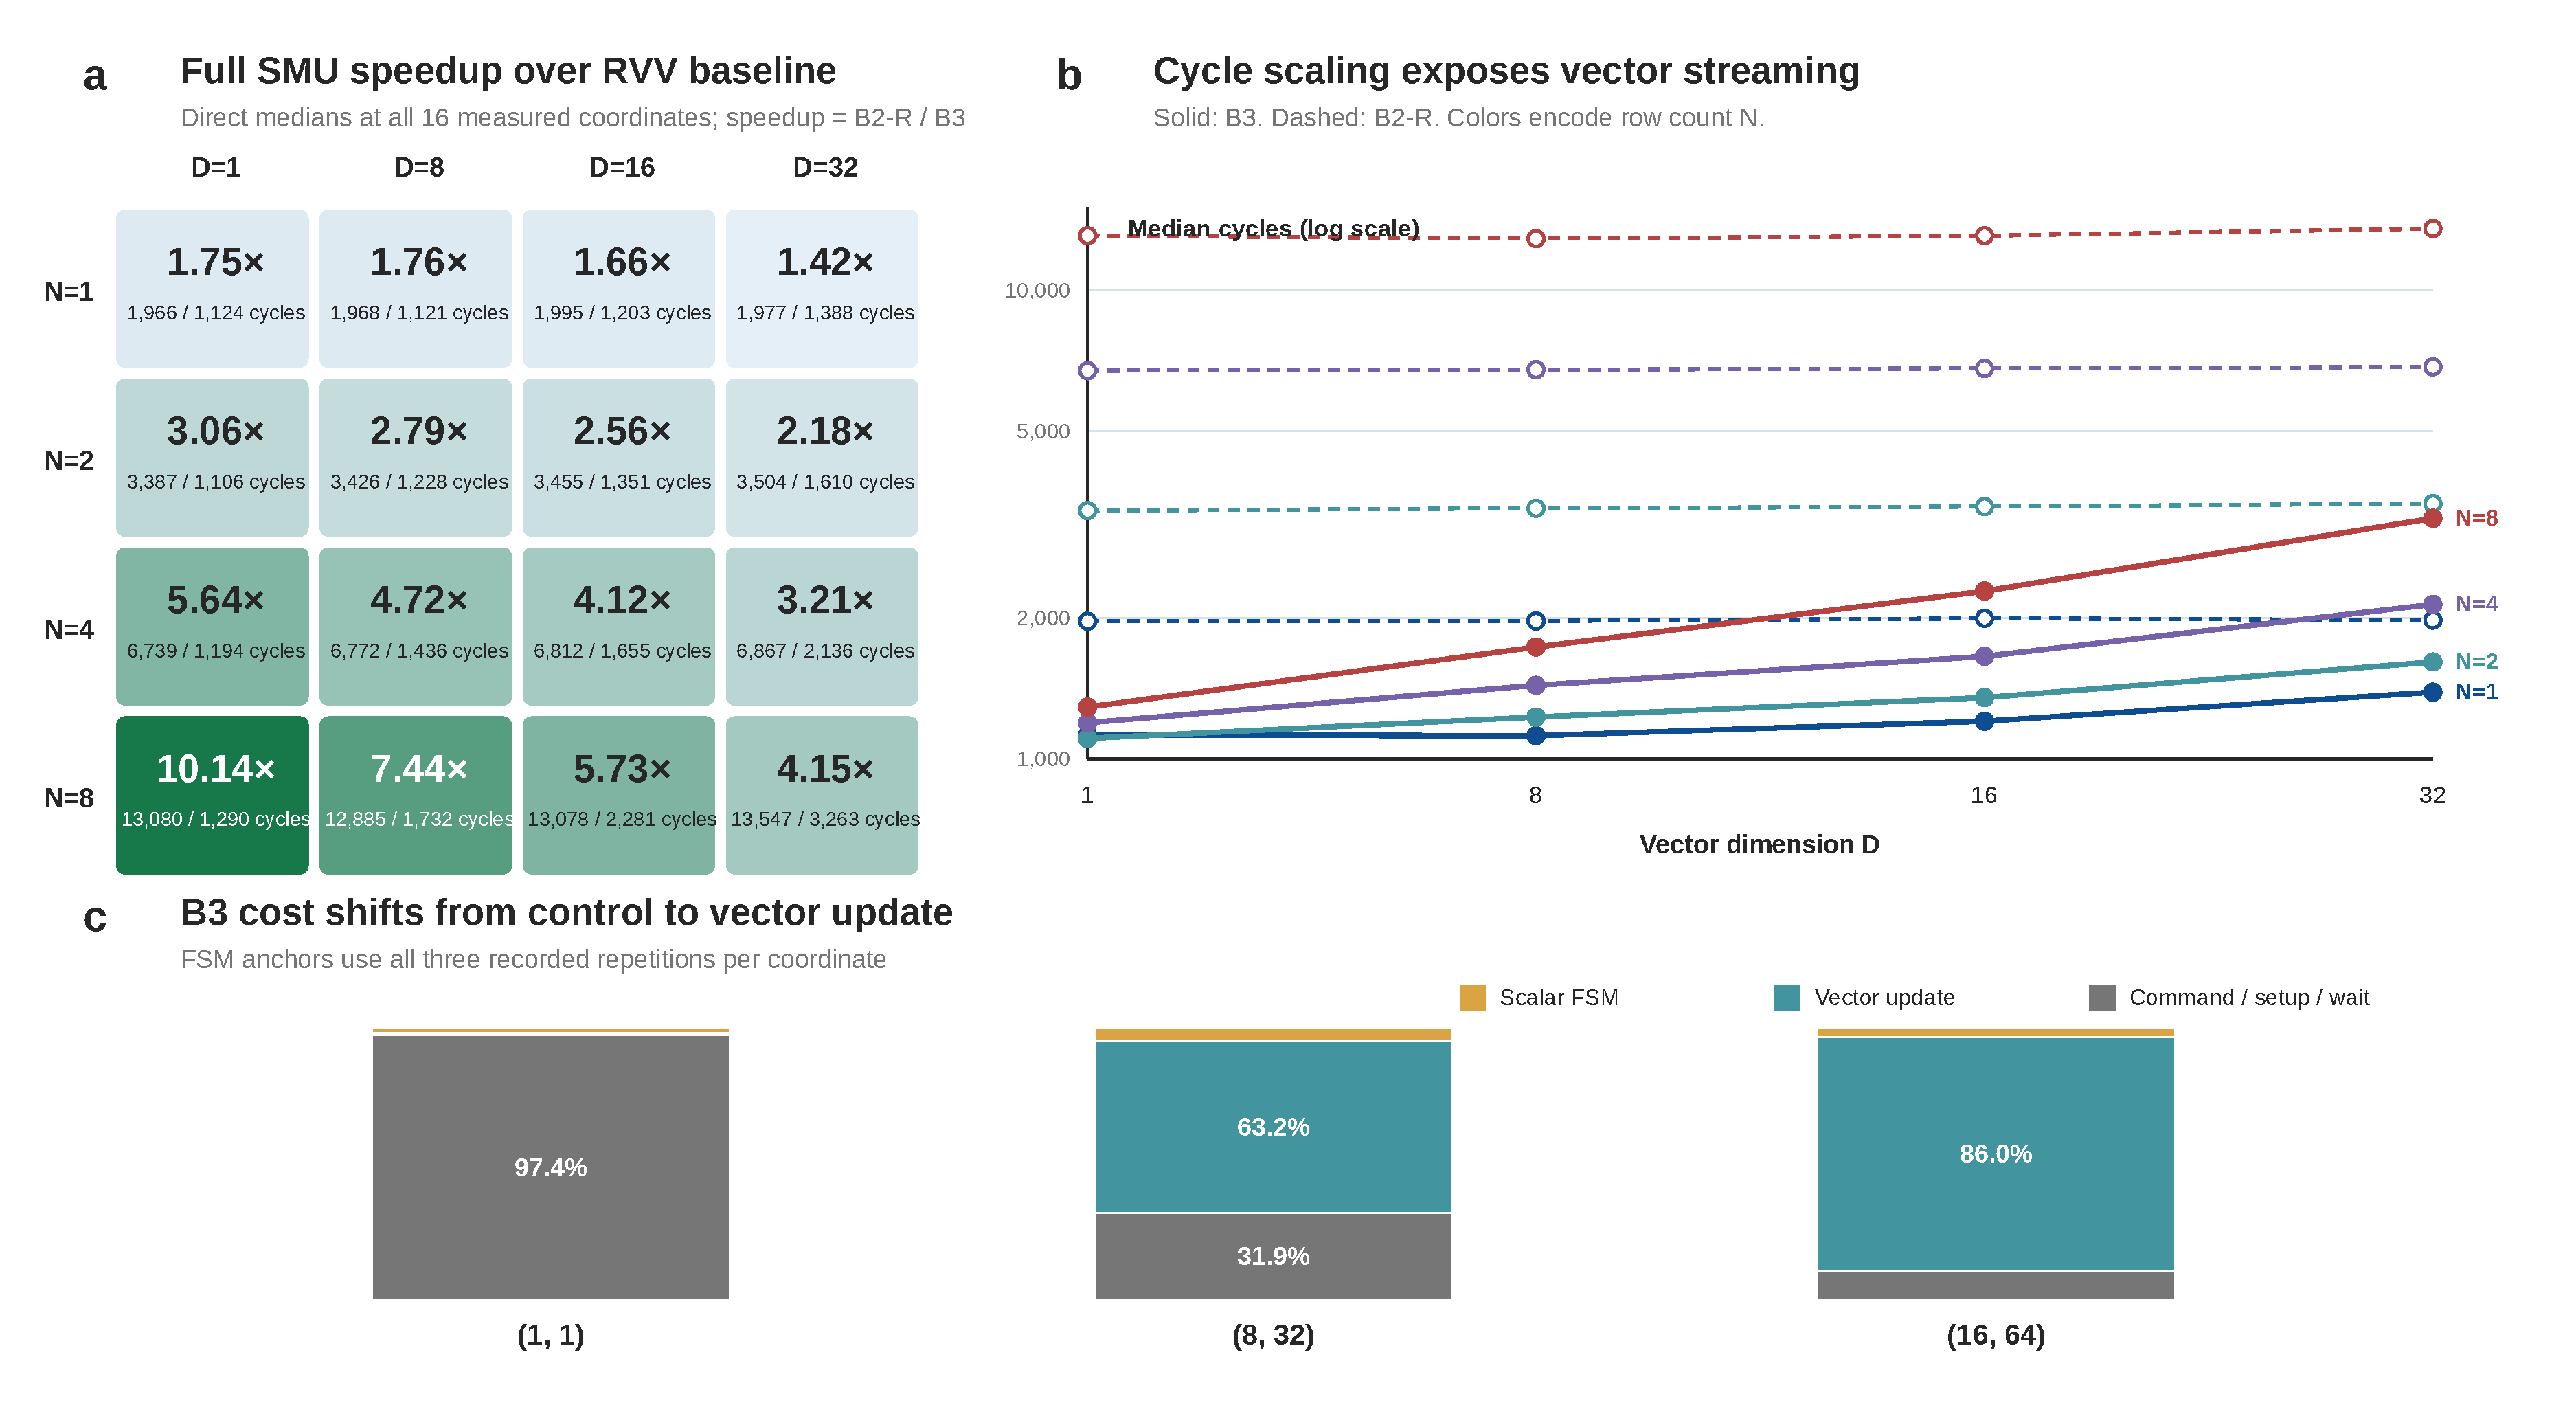
\includegraphics[width=0.97\textwidth]{figures/smu_scaling_bottleneck.pdf}
\caption{SMU scaling and bottleneck transition. (a) Full SMU speedup over the
RTL-aligned RVV baseline at all 16 direct measurement coordinates. Each cell
reports median B2-R/B3 cycles. (b) Absolute B2-R and B3 cycle scaling across
every row count and vector dimension. (c) End-to-end B3 cycle decomposition at
the three recorded FSM anchors. The command/setup/wait share dominates at
$(1,1)$, while vector update dominates at larger coordinates.}
\label{fig:scaling-bottleneck}
\end{figure*}

The full mixed-scalar sweep supplies a second reference point. It compares B3
with B1 and reaches 37.89$\times$ at $(16,64)$. This value uses a scalar
reference and does not replace the stricter B2-R comparison in
Figure~\ref{fig:scaling-bottleneck}.

\begin{table}[t]
\caption{Representative measured cycle counts. B1 and B2-R execute software;
B3 executes the full SMU.}
\label{tab:cycles}
\centering\small
\renewcommand{\arraystretch}{1.06}
\begin{tabular}{c|r|r|r|r}
\toprule
$(N,D)$ & B1 & B2-R & B3 & B2-R/B3\\
\midrule
$(1,1)$ & 2,530 & 1,966 & 1,124 & 1.75$\times$\\
$(4,8)$ & 17,900 & 6,772 & 1,436 & 4.72$\times$\\
$(8,32)$ & 99,794 & 13,547 & 3,263 & 4.15$\times$\\
$(16,64)$ & 371,610 & 27,532 & 9,556 & 2.88$\times$\\
\bottomrule
\end{tabular}
\end{table}

\subsection{The bottleneck moves from control to vector streaming}

The controller spends 1,095 of 1,124 end-to-end cycles outside SMU busy time
at $(1,1)$. At $(8,32)$, vector update consumes 2,063 of 2,223 busy cycles.
At $(16,64)$, vector update consumes 8,214 of 8,534 busy cycles. The scalar
portion falls from 69\% to 3.7\% of busy cycles across these coordinates. The
engine removes the original row-level scalar bottleneck, then exposes the
streaming update as the dominant optimization target.

The phase counts also guide a hardware roadmap. Small operations need a lower
cost launch and completion interface because fixed command work dominates
their end-to-end time. Larger operations need more vector bandwidth, wider
datapaths, or multiple engines because the current scalar mechanism already
consumes a small share of active cycles. The current controller makes this
tradeoff visible without changing the core pipeline.

\subsection{Shared TCDM preserves component throughput}

Across all 16 bank phases at $(16,64)$, the concurrent B3 execution records a
median 8,533 SMU busy cycles versus 8,529 standalone cycles. The paired core
workload records 3,163 cycles versus 3,144 standalone cycles. Median TCDM
congestion reaches 1.27\%, and concurrent execution saves 1,447 cycles over
serial execution. The result shows useful overlap on this cluster, while it
does not establish throughput for a complete attention kernel.

The bank-phase sweep produces a narrow range of total concurrent time from
10,184 to 10,235 cycles. This range shows that bank placement affects the
observed overlap but does not alter the conclusion for the tested workload.
The experiment uses one engine and one core stream. Additional cores, engines,
or a full attention schedule can create a different contention regime.

\subsection{Accuracy remains bounded on recorded merge cases}

The LUT model evaluates the full recurrence over generic mixed inputs and a
delta sweep. Its largest recorded absolute error is $9.78\times10^{-6}$ at
$(16,64)$, and its largest guarded relative error is
$3.33\times10^{-6}$. The model uses 256 interpolation segments for both
exponential and reciprocal tables. These values characterize the selected LUT
construction before the engine introduces fixed-point conversion and streaming
state updates.

The RTL comparison measures that complete implementation. The largest recorded
absolute error in the FSM analysis is $6.03\times10^{-4}$ at $(8,32)$, and the
largest recorded relative error is $1.61\times10^{-4}$ at $(16,64)$. Each
reported B2-R and B3 repetition passes the benchmark threshold of $10^{-3}$.
The difference between the model and RTL values reflects the fixed-point
arithmetic that the hardware datapath uses to form scaled lengths and weighted
vector terms. The result provides a measured validation boundary for the
present implementation rather than a claim about every attention input.

We also execute an attention-like merge chain with eight rows, four blocks,
and $D=32$. This workload performs successive SMU merges over 1,024 vector
elements and records 13,432 engine cycles versus 388,826 cycles for its
RTL-aligned scalar reference. It exercises the same $m$, $l$, and $O$ state
flow that tiled attention needs after partial results become available. It
excludes QK scoring, PV accumulation, masking, DRAM traffic, and runtime
scheduling. The chain therefore extends the microbenchmark evidence without
becoming an end-to-end attention result.

\begin{table}[t]
\caption{Numerical and exploratory implementation evidence.}
\label{tab:evidence}
\centering\small
\renewcommand{\arraystretch}{1.08}
\begin{tabular}{p{0.26\columnwidth}p{0.62\columnwidth}}
\toprule
Evidence & Observation\\
\midrule
LUT model & Worst absolute error $9.78\times10^{-6}$ across recorded cases.\\
RTL checks & Maximum observed absolute error $6.03\times10^{-4}$ at $(8,32)$; all recorded checks pass the $10^{-3}$ threshold.\\
Generic logic proxy & Full SMU maps to 94,713 post-techmap generic cells in Yosys.\\
Toggle proxy & At $(16,64)$, B3 records 12.5M zero-delay toggles versus 41.5M for B2-R.\\
\bottomrule
\end{tabular}
\end{table}

\section{Discussion}

\subsection{The design targets a specific granularity}

The SMU receives a complete merge command, so each launch carries a fixed
configuration and completion cost. The measurements show that this choice
works best when several rows amortize that cost. At $(1,1)$, only 29 SMU busy
cycles execute inside a 1,124-cycle end-to-end operation. At $(16,64)$, the
engine executes 8,534 busy cycles inside 9,556 end-to-end cycles. This change
explains why the engine remains useful for matrix shapes that contain many
short scalar recurrences, even when each recurrence has a compact vector.

The command boundary also defines a clear deployment path. A tiled attention
kernel can retain its QK and PV computation on an existing vector or matrix
engine, place the partial $(m,l,O)$ state in local scratchpad memory, and
submit merge commands at tile completion. The current prototype serializes one
command, but independent rows and heads expose natural opportunities for
multiple engines. A future front end can batch commands or use a queue to
reduce the small-workload overhead that the current MMIO protocol reveals.

\subsection{The evaluation distinguishes evidence layers}

The paper uses three measurement layers because each answers a separate
question. RTL end-to-end cycles establish the software-versus-engine result.
FSM counters establish where the engine spends active cycles. The concurrency
experiment establishes whether a co-running stream alters those component
times. The combination gives a stronger explanation than a speedup number
alone: the scalar work leaves the core, the vector loop becomes dominant, and
the shared scratchpad introduces measurable yet small interference for the
tested stream.

The numerical results also have two layers. The host model tests the selected
LUT interpolation and reciprocal construction against the complete recurrence.
The RTL benchmark tests the implemented fixed-point data path against its
RTL-aligned software reference. Reporting both values prevents the lower model
error from becoming an end-to-end RTL claim. The explicit validation paths
serve the same purpose. They show that the engine rejects malformed commands
instead of silently producing an output.

\subsection{Proxy data guides follow-up work}

The generic logic and toggle measurements guide architectural choices but do
not replace physical implementation. The resource decomposition assigns most
generic cells to the vector arithmetic and data path, while the exponential and
reciprocal blocks occupy smaller independent scopes. The toggle traces show a
lower count for B3 at the largest sampled coordinate because B3 completes the
operation in fewer target cycles. These observations motivate vector-path
optimization and physical synthesis. They do not establish an area, frequency,
power, or energy advantage.

\section{Limitations and Related Work}

Online normalization provides the recurrence that enables streaming softmax
state \cite{milakov2018online}. IO-aware attention algorithms use this
structure to process tiles without materializing full score matrices
\cite{dao2022flashattention}. The \smu{} complements these algorithms at the
cluster level. It accelerates the merge state after a tile; it does not
implement QK multiplication, PV multiplication, masking, scheduling, or an
end-to-end attention runtime.

Spatz supplies compact vector execution and a shared scratchpad
\cite{spatz2023}. Our design adds a TCDM master beside this execution path
instead of introducing a vector instruction. The evaluation compares
RTL-aligned software paths, not an optimized CPU, GPU, or production attention
kernel. The Yosys and toggle numbers remain logic-activity proxies. A physical
technology library, timing constraints, and power analysis would be required
for PPA claims.

The approximation range also bounds the current result. The exponential LUT
saturates below $-8$ and above zero, and the input validation excludes NaN,
infinity, and subnormal values. The measured numerical cases cover mixed
scalar inputs, a delta sweep, and a merge-chain workload. They establish
behavior for those cases; they do not provide a universal error bound over all
attention distributions. A future design can add wider approximation ranges,
refinement steps, or IEEE floating-point datapaths when the target workload
requires them.

\section{Conclusion}

The SMU moves online-softmax merge state updates into a compact TCDM-connected
engine while preserving the Spatz ISA and vector pipeline. Measured B3 results
outperform the RTL-aligned RVV-assisted baseline at all 16 scaling coordinates
and retain component throughput during a shared-TCDM experiment. The measured
FSM phases identify vector streaming and command overhead as the next design
targets. These results establish cluster-local merge offload as a practical
building block for future tiled-attention systems.

\bibliographystyle{IEEEtran}
\bibliography{refs}
\end{document}
